\documentclass{standalone}
\usepackage{tikz}
\usetikzlibrary{patterns, positioning}


\begin{document}
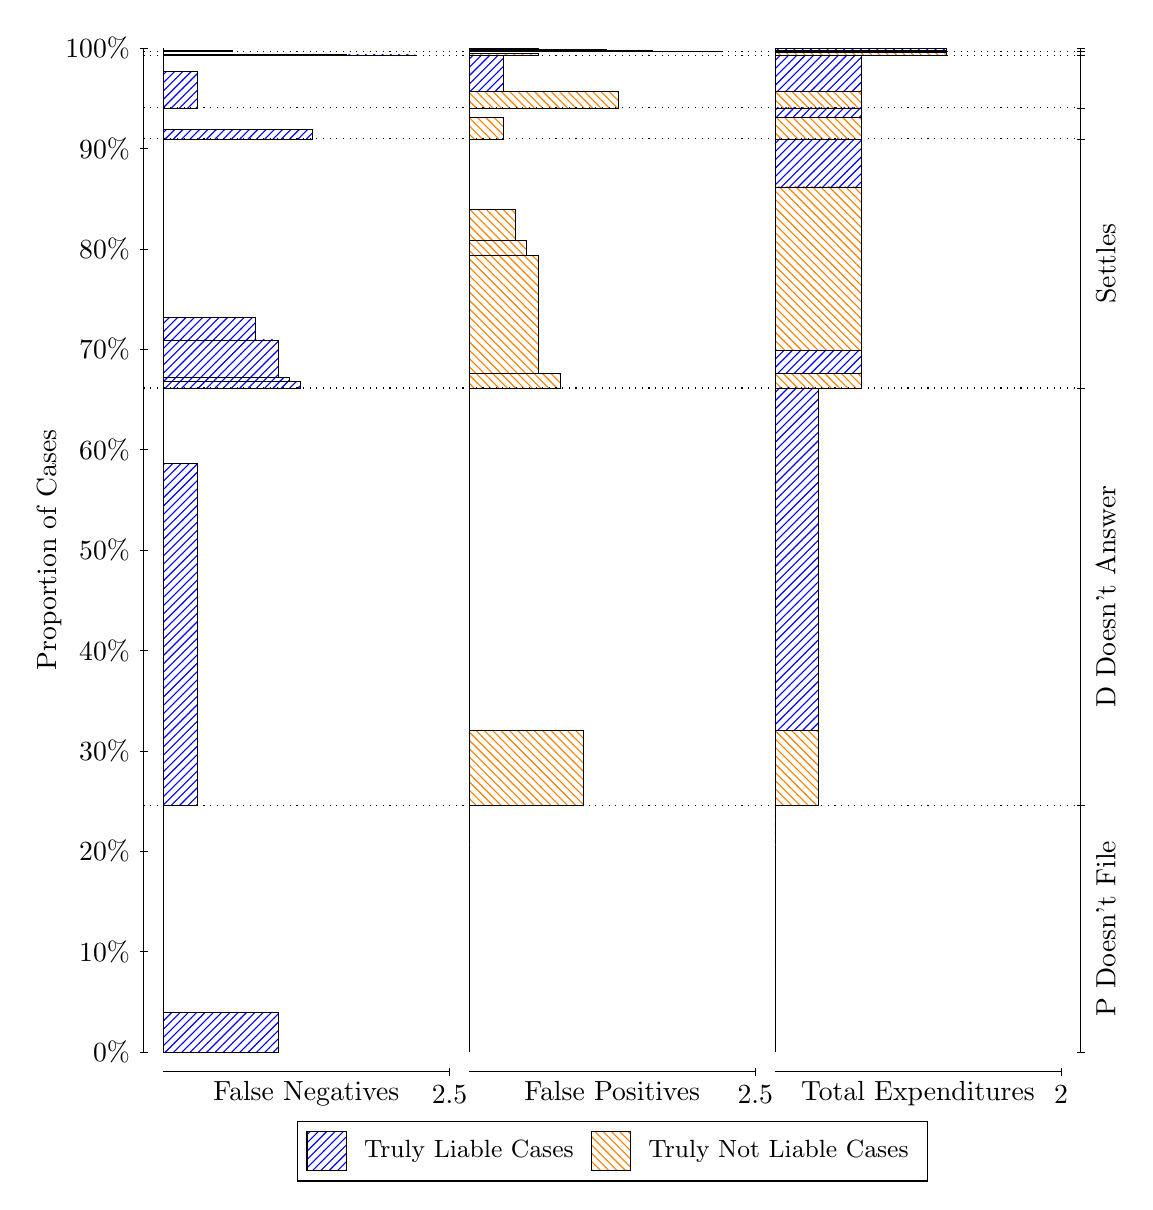
\begin{tikzpicture}
\draw[black, very thin] (1.5,1.75) -- (1.5,14.5);
\node[rotate=90, text=black, anchor=center] at (0.3, 8.125) {Proportion of Cases};
\draw[black, very thin] (1.45,1.75) -- (1.55,1.75);
\node[text=black, anchor=east] at (1.45, 1.75) {0\%};
\draw[black, very thin] (1.45,3.025) -- (1.55,3.025);
\node[text=black, anchor=east] at (1.45, 3.025) {10\%};
\draw[black, very thin] (1.45,4.3) -- (1.55,4.3);
\node[text=black, anchor=east] at (1.45, 4.3) {20\%};
\draw[black, very thin] (1.45,5.575) -- (1.55,5.575);
\node[text=black, anchor=east] at (1.45, 5.575) {30\%};
\draw[black, very thin] (1.45,6.85) -- (1.55,6.85);
\node[text=black, anchor=east] at (1.45, 6.85) {40\%};
\draw[black, very thin] (1.45,8.125) -- (1.55,8.125);
\node[text=black, anchor=east] at (1.45, 8.125) {50\%};
\draw[black, very thin] (1.45,9.4) -- (1.55,9.4);
\node[text=black, anchor=east] at (1.45, 9.4) {60\%};
\draw[black, very thin] (1.45,10.675) -- (1.55,10.675);
\node[text=black, anchor=east] at (1.45, 10.675) {70\%};
\draw[black, very thin] (1.45,11.95) -- (1.55,11.95);
\node[text=black, anchor=east] at (1.45, 11.95) {80\%};
\draw[black, very thin] (1.45,13.225) -- (1.55,13.225);
\node[text=black, anchor=east] at (1.45, 13.225) {90\%};
\draw[black, very thin] (1.45,14.5) -- (1.55,14.5);
\node[text=black, anchor=east] at (1.45, 14.5) {100\%};

\draw[black, very thin] (13.4,1.75) -- (13.4,14.5);
\draw[black, very thin] (13.35,1.75) -- (13.45,1.75);
\node[anchor=west] at (13.35, 1.75) {};
\draw[black, very thin] (13.35,4.8833) -- (13.45,4.8833);
\node[anchor=west] at (13.35, 4.8833) {};
\draw[black, very thin] (13.35,10.183) -- (13.45,10.183);
\node[anchor=west] at (13.35, 10.183) {};
\draw[black, very thin] (13.35,13.346) -- (13.45,13.346);
\node[anchor=west] at (13.35, 13.346) {};
\draw[black, very thin] (13.35,13.741) -- (13.45,13.741);
\node[anchor=west] at (13.35, 13.741) {};
\draw[black, very thin] (13.35,14.409) -- (13.45,14.409);
\node[anchor=west] at (13.35, 14.409) {};
\draw[black, very thin] (13.35,14.456) -- (13.45,14.456);
\node[anchor=west] at (13.35, 14.456) {};
\draw[black, very thin] (13.35,14.5) -- (13.45,14.5);
\node[anchor=west] at (13.35, 14.5) {};

\draw[black, very thin, pattern color=blue, pattern=north east lines] (1.75,1.75) rectangle (3.2033,2.2496);
\draw[black, very thin, pattern color=orange, pattern=north west lines] (1.75,2.2496) rectangle (1.75,4.8833);
\draw[black, very thin, pattern color=blue, pattern=north east lines] (1.75,4.8833) rectangle (2.186,9.2285);
\draw[black, very thin, pattern color=orange, pattern=north west lines] (1.75,9.2285) rectangle (1.75,10.183);
\draw[black, very thin, pattern color=blue, pattern=north east lines] (1.75,10.183) rectangle (3.494,10.268);
\draw[black, very thin, pattern color=blue, pattern=north east lines] (1.75,10.268) rectangle (3.3487,10.313);
\draw[black, very thin, pattern color=blue, pattern=north east lines] (1.75,10.313) rectangle (3.2033,10.793);
\draw[black, very thin, pattern color=blue, pattern=north east lines] (1.75,10.793) rectangle (2.9127,11.083);
\draw[black, very thin, pattern color=orange, pattern=north west lines] (1.75,11.083) rectangle (1.75,13.346);
\draw[black, very thin, pattern color=blue, pattern=north east lines] (1.75,13.346) rectangle (3.6393,13.467);
\draw[black, very thin, pattern color=orange, pattern=north west lines] (1.75,13.467) rectangle (1.75,13.741);
\draw[black, very thin, pattern color=blue, pattern=north east lines] (1.75,13.741) rectangle (2.186,14.205);
\draw[black, very thin, pattern color=orange, pattern=north west lines] (1.75,14.205) rectangle (1.75,14.409);
\draw[black, very thin, pattern color=blue, pattern=north east lines] (1.75,14.409) rectangle (4.9473,14.413);
\draw[black, very thin, pattern color=blue, pattern=north east lines] (1.75,14.413) rectangle (4.0753,14.424);
\draw[black, very thin, pattern color=orange, pattern=north west lines] (1.75,14.424) rectangle (1.75,14.456);
\draw[black, very thin, pattern color=blue, pattern=north east lines] (1.75,14.456) rectangle (2.622,14.473);
\draw[black, very thin, pattern color=orange, pattern=north west lines] (1.75,14.473) rectangle (1.75,14.488);
\draw[black, very thin, pattern color=blue, pattern=north east lines] (1.75,14.488) rectangle (1.75,14.5);
\draw[black, very thin, pattern color=orange, pattern=north west lines] (5.6333,1.75) rectangle (5.6333,4.3837);
\draw[black, very thin, pattern color=blue, pattern=north east lines] (5.6333,4.3837) rectangle (5.6333,4.8833);
\draw[black, very thin, pattern color=orange, pattern=north west lines] (5.6333,4.8833) rectangle (7.0867,5.8375);
\draw[black, very thin, pattern color=blue, pattern=north east lines] (5.6333,5.8375) rectangle (5.6333,10.183);
\draw[black, very thin, pattern color=orange, pattern=north west lines] (5.6333,10.183) rectangle (6.796,10.37);
\draw[black, very thin, pattern color=orange, pattern=north west lines] (5.6333,10.37) rectangle (6.5053,11.862);
\draw[black, very thin, pattern color=orange, pattern=north west lines] (5.6333,11.862) rectangle (6.36,12.061);
\draw[black, very thin, pattern color=orange, pattern=north west lines] (5.6333,12.061) rectangle (6.2147,12.446);
\draw[black, very thin, pattern color=blue, pattern=north east lines] (5.6333,12.446) rectangle (5.6333,13.346);
\draw[black, very thin, pattern color=orange, pattern=north west lines] (5.6333,13.346) rectangle (6.0693,13.619);
\draw[black, very thin, pattern color=blue, pattern=north east lines] (5.6333,13.619) rectangle (5.6333,13.741);
\draw[black, very thin, pattern color=orange, pattern=north west lines] (5.6333,13.741) rectangle (7.5227,13.946);
\draw[black, very thin, pattern color=blue, pattern=north east lines] (5.6333,13.946) rectangle (6.0693,14.409);
\draw[black, very thin, pattern color=orange, pattern=north west lines] (5.6333,14.409) rectangle (6.5053,14.428);
\draw[black, very thin, pattern color=orange, pattern=north west lines] (5.6333,14.428) rectangle (5.6333,14.441);
\draw[black, very thin, pattern color=blue, pattern=north east lines] (5.6333,14.441) rectangle (5.6333,14.456);
\draw[black, very thin, pattern color=orange, pattern=north west lines] (5.6333,14.456) rectangle (8.8307,14.459);
\draw[black, very thin, pattern color=orange, pattern=north west lines] (5.6333,14.459) rectangle (7.9587,14.47);
\draw[black, very thin, pattern color=blue, pattern=north east lines] (5.6333,14.47) rectangle (7.3773,14.483);
\draw[black, very thin, pattern color=blue, pattern=north east lines] (5.6333,14.483) rectangle (6.5053,14.5);
\draw[black, very thin, pattern color=orange, pattern=north west lines] (9.5167,1.75) rectangle (9.5167,4.3837);
\draw[black, very thin, pattern color=blue, pattern=north east lines] (9.5167,4.3837) rectangle (9.5167,4.8833);
\draw[black, very thin, pattern color=orange, pattern=north west lines] (9.5167,4.8833) rectangle (10.062,5.8375);
\draw[black, very thin, pattern color=blue, pattern=north east lines] (9.5167,5.8375) rectangle (10.062,10.183);
\draw[black, very thin, pattern color=orange, pattern=north west lines] (9.5167,10.183) rectangle (10.607,10.37);
\draw[black, very thin, pattern color=blue, pattern=north east lines] (9.5167,10.37) rectangle (10.607,10.66);
\draw[black, very thin, pattern color=orange, pattern=north west lines] (9.5167,10.66) rectangle (10.607,12.736);
\draw[black, very thin, pattern color=blue, pattern=north east lines] (9.5167,12.736) rectangle (10.607,13.346);
\draw[black, very thin, pattern color=orange, pattern=north west lines] (9.5167,13.346) rectangle (10.607,13.619);
\draw[black, very thin, pattern color=blue, pattern=north east lines] (9.5167,13.619) rectangle (10.607,13.741);
\draw[black, very thin, pattern color=orange, pattern=north west lines] (9.5167,13.741) rectangle (10.607,13.946);
\draw[black, very thin, pattern color=blue, pattern=north east lines] (9.5167,13.946) rectangle (10.607,14.409);
\draw[black, very thin, pattern color=orange, pattern=north west lines] (9.5167,14.409) rectangle (11.697,14.441);
\draw[black, very thin, pattern color=blue, pattern=north east lines] (9.5167,14.441) rectangle (11.697,14.456);
\draw[black, very thin, pattern color=orange, pattern=north west lines] (9.5167,14.456) rectangle (11.697,14.47);
\draw[black, very thin, pattern color=blue, pattern=north east lines] (9.5167,14.47) rectangle (11.697,14.5);
\draw[black, dotted] (1.5,4.8833) -- (13.4,4.8833);
\draw[black, dotted] (1.5,10.183) -- (13.4,10.183);
\draw[black, dotted] (1.5,13.346) -- (13.4,13.346);
\draw[black, dotted] (1.5,13.741) -- (13.4,13.741);
\draw[black, dotted] (1.5,14.409) -- (13.4,14.409);
\draw[black, dotted] (1.5,14.456) -- (13.4,14.456);
\draw[black, very thin] (1.75,1.5) -- (5.3833,1.5);
\node[text=black, anchor=north] at (3.5667, 1.5) {False Negatives};
\draw[black, very thin] (5.3833,1.45) -- (5.3833,1.55);
\node[text=black, anchor=north] at (5.3833, 1.45) {2.5};

\draw[black, very thin] (5.6333,1.5) -- (9.2667,1.5);
\node[text=black, anchor=north] at (7.45, 1.5) {False Positives};
\draw[black, very thin] (9.2667,1.45) -- (9.2667,1.55);
\node[text=black, anchor=north] at (9.2667, 1.45) {2.5};

\draw[black, very thin] (9.5167,1.5) -- (13.15,1.5);
\node[text=black, anchor=north] at (11.333, 1.5) {Total Expenditures};
\draw[black, very thin] (13.15,1.45) -- (13.15,1.55);
\node[text=black, anchor=north] at (13.15, 1.45) {2};

\node[text=black, centered, rotate=90] at (13.72, 3.3166) {P Doesn't File};
\node[text=black, centered, rotate=90] at (13.72, 7.533) {D Doesn't Answer};
\node[text=black, centered, rotate=90] at (13.72, 11.764) {Settles};





\draw (7.449999999999999,1.5) node[draw=none] (baseCoordinate) {};
\begin{scope}[align=center]
        \matrix[scale=0.5, draw=black, below=0.5cm of baseCoordinate, nodes={draw}, column sep=0.1cm]{
            \node[rectangle, draw, minimum width=0.5cm, minimum height=0.5cm, pattern color=blue, pattern=north east lines] {}; &
            \node[draw=none, font=\small, text=black] (B) {Truly Liable Cases}; &
            \node[rectangle, draw, minimum width=0.5cm, minimum height=0.5cm, pattern color=orange, pattern=north west lines] {}; &
            \node[draw=none, font=\small, text=black] (B) {Truly Not Liable Cases}; \\
            };
\end{scope}

\end{tikzpicture}
\end{document}